\item It is given that $\vec{X}_1, \vec{X}_2, \ldots, \vec{X}_M$ are $M$ non-zero, orthogonal vectors. The dimension of the vector space spanned by the $2M$ vectors $\vec{X}_1, \vec{X}_2, \ldots, \vec{X}_M, -\vec{X}_1, -\vec{X}_2, \ldots, -\vec{X}_M$ is
\hfill{(EC 2007)}
\begin{enumerate}
	\begin{multicols}{2}
    \item $2M$
    \item $M+1$
    \item $M$
    \item \text{Dependent on choice of } $X_i$
    \end{multicols}
\end{enumerate}
%
\item Three functions $f_1\brak{t}, f_2\brak{t}$ and $f_3\brak{t}$, which are zero outside the interval $[0,7]$, are shown in the figure. Which of the following statements is correct? 
\hfill{(EC 2007)}
\begin{figure}[H]
    \centering
    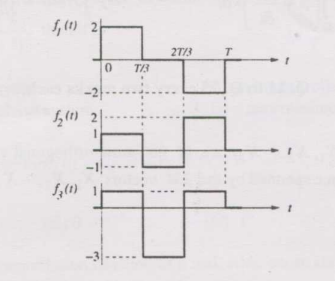
\includegraphics[width=0.7\columnwidth]{GATE/2007/EC/figs/Q26.png}
    \caption{}
    \label{fig:Q26.png}
\end{figure}
\begin{enumerate}
	\begin{multicols}{2}
    \item $f_1\brak{t}$ and $f_2\brak{t}$ are orthogonal
    \item $f_1\brak{t}$ and $f_3\brak{t}$ are orthogonal
    \item $f_2\brak{t}$ and $f_3\brak{t}$ are orthogonal
    \item $f_1\brak{t}$ and $f_2\brak{t}$ are orthonormal
    \end{multicols}
\end{enumerate}
%
\item  Consider a linear system whose state space representation is $\dot{x}\brak{t} = \vec{A} x\brak{t}$.
If the initial state vector of the system is $\vec{x}\brak{0} = \myvec{1 \\ -2}$, then the system response is 
$\vec{x}\brak{t} = \myvec{e^{-2t}  -2e^{-2t}}.$ 
If the initial state vector of the system changes to $\vec{x}\brak{0} = \myvec{1  \\ -1}$,
then the system response becomes $\vec{x}\brak{t} = \myvec{e^{-t}  -e^{-t}}$. 
\begin{enumerate}
\item The eigenvalue and eigenvector pairs  for the system are
\hfill{\brak{(EC 2007)}}
%
\begin{enumerate}
\begin{multicols}{2}
  \item $\brak{-1,\myvec{1 \\ -1}}$ and $\brak{-2, \myvec{1 \\ -2}}$
  \item $\brak{-2,\myvec{1 \\ -1}}$ and $\brak{-1, \myvec{1 \\ -2}}$
  \item $\brak{-1,\myvec{1 \\ -1}}$ and $\brak{2,\myvec{1 \\ -2}}$
  \item $\brak{-2,\myvec{1 \\ -1}}$ and $\brak{1,\myvec{1 \\ -2}}$
  \end{multicols}
\end{enumerate}
% 
\item The system matrix $\vec{A}$ is  
\hfill{\brak{(EC 2007)}}
\begin{multicols}{4}
\begin{enumerate}
  \item $\myvec{0 & 1 \\ -1 & 1}$
  \item $\myvec{1 & 1 \\ -1 & -2}$
  \item $\myvec{2 & 1 \\ -1 & -1}$
  \item $\myvec{0 & 1 \\ -2 & -3}$
\end{enumerate}
\end{multicols}
\end{enumerate}

